\documentclass{sig-alternate}

\usepackage[usenames,dvipsnames]{color}
\usepackage{xspace}

\usepackage{fancyvrb}
\DefineVerbatimEnvironment{code}{Verbatim}{fontsize=\small}
\DefineVerbatimEnvironment{example}{Verbatim}{fontsize=\small}

% Looks better (and more concise) than Times New Roman
\usepackage{times}
% Better spacing
\usepackage{microtype}
\usepackage[normalem]{ulem}
\usepackage{enumitem}
% Caption package both lets you set the spacing between figure and caption
% and also makes the \figref{} point to the right place.
\usepackage[font=bf,aboveskip=0pt,belowskip=-12pt]{caption}
% Get the caption package to work with ACM style
\DeclareCaptionType[placement=b,within=none]{copyrightbox}
%%%%%%%%%%%%%%%%%%%%%%%%%%%%%%%%%%%%%%%%%%%%%%%%%%%%%%%%%%%%%%%%%%%%%
\newfont{\mycrnotice}{ptmr8t at 7pt}
\newfont{\myconfname}{ptmri8t at 7pt}
\let\crnotice\mycrnotice%
\let\confname\myconfname%

\permission{Permission to make digital or hard copies of all or part of this work for personal or classroom use is granted without fee provided that copies are not made or distributed for profit or commercial advantage and that copies bear this notice and the full citation on the first page. Copyrights for components of this work owned by others than the author(s) must be honored. Abstracting with credit is permitted. To copy otherwise, or republish, to post on servers or to redistribute to lists, requires prior specific permission and/or a fee. Request permissions from Permissions@acm.org.}
\conferenceinfo{}{DMAH 2015, September 4th, Kohala Coast, USA}
\copyrightetc{}
\crdata{}

% Allow comments by name
\newcommand{\note}[2]{
    \textbf{\textcolor{#1}{#2}}
}
\newcommand{\comment}[1]{\note{red}{#1}}
\newcommand{\dave}[1]{\note{PineGreen}{Dave: #1}}
\newcommand{\magda}[1]{\note{Cyan}{Magda: #1}}
\newcommand{\tom}[1]{\note{OrangeRed}{Tom: #1}}

% To remove all notes, uncomment the next line.
%\renewcommand{\note}[2]{\unskip}

\newcommand{\ie}{{\em i.e.}\ }
\newcommand{\eg}{{\em e.g.}\ }
\newcommand{\ea}{{\em et al.}\xspace}
\newcommand{\aka}{{\em a.k.a.}\ }

\usepackage{url}
\usepackage[pdftex]{hyperref}

% Figures
\newcommand{\figureimgs}{
\begin{figure}[tbp]
  \centering
  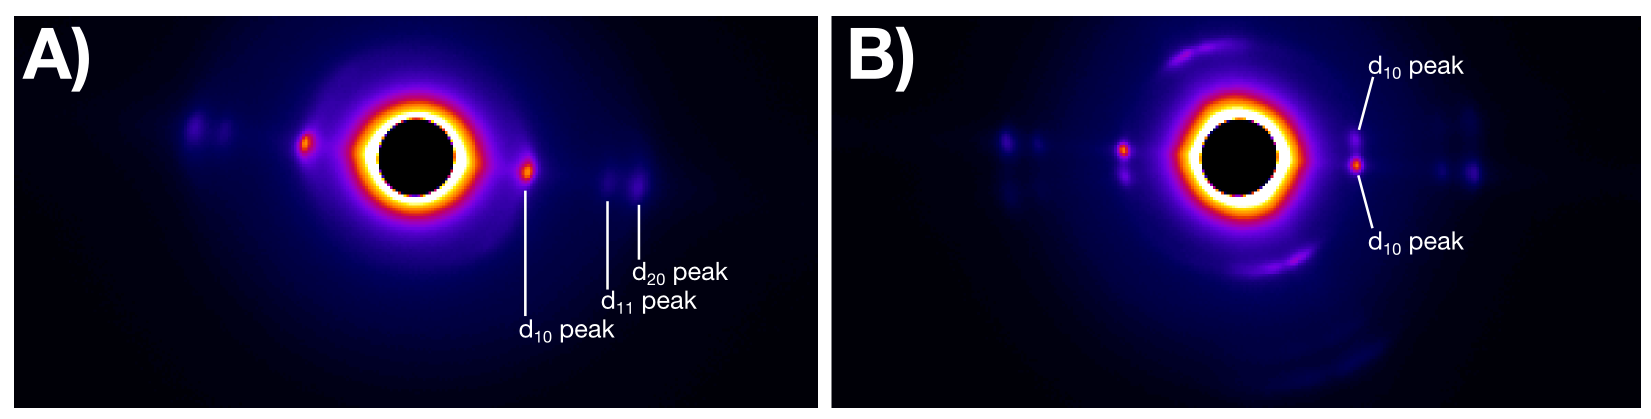
\includegraphics[width=\linewidth]{figures/x_ray_image_montage}
  \vspace{-12pt}
  \caption{\label{fig:imgs}
  	X-ray diffraction images.
    A) An X-ray diffraction image exhibits $d_{10}$, $d_{11}$, and
    $d_{20}$ peaks; the first and last are proportional to the
    distance between adjacent rows of thick filaments. The $d_{10}$ is
    the primary peak being targeted for automated detection and
    fitting. B) In this image, two fibers at slight angles to each
    other have generated multiple $d_{10}$ peaks which must be
    segregated during the detection process.  
	}
	\vspace{-2pt}
\end{figure}
}

\newcommand{\figureworkflow}{
\begin{figure}[tbp]
  \centering
  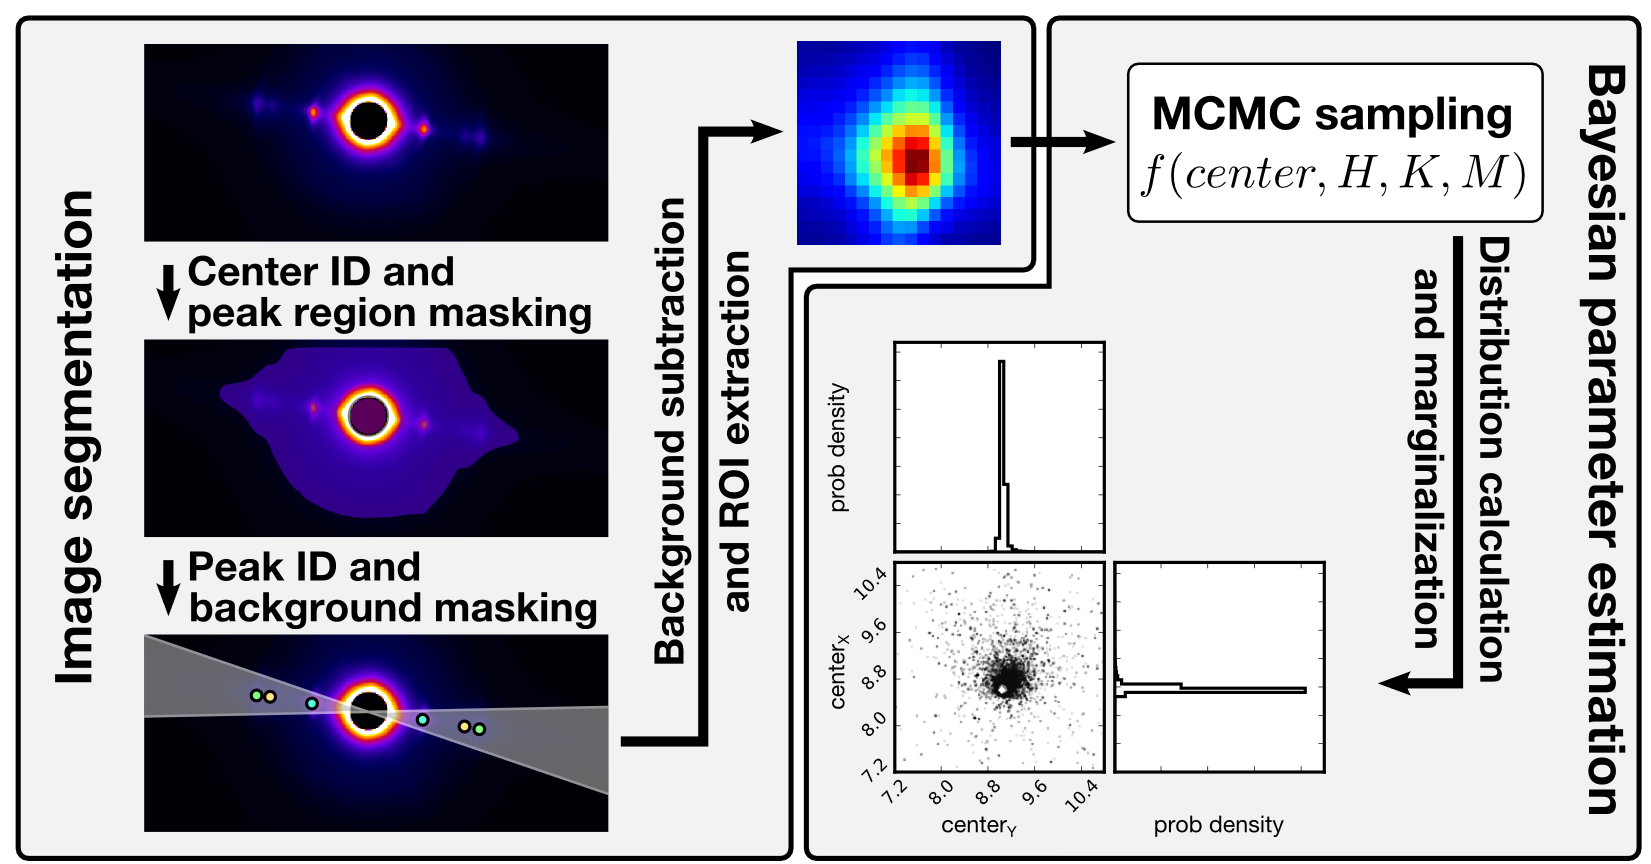
\includegraphics[width=\linewidth]{figures/img_analysis}
  \vspace{-8pt}
  \caption{\label{fig:workflow}
  	Analysis workflow.
    The blocked center region is detected and used for registration.
    Low signal regions and edges are masked. The image is smoothed and
    peaks are detected, clustered, and classified. The background
    (minus that surrounding diffraction lines) is computed and
    subtracted. Regions of interest surrounding the $d_{10}$ peaks are
    extracted and the generating distributions are fit with an MCMC
    sampler. We marginalize across peak parameters other than those of
    interest.  
	}
	\vspace{-2pt}
\end{figure}
}

\begin{document}
\title{Automated analysis of muscle X-ray diffraction \\ imaging with MCMC}
\author{C.\ David Williams$^{1,2}$,  Magdalena Balazinska$^2$, Thomas Daniel$^1$ \\
\affaddr{$^1$Department of Biology, $^2$Department of Computer Science \& Engineering}\\
\affaddr{University of Washington} \\
}
\maketitle



% \dave{Presumably this gets filled in later?}
%    \vspace{-8pt}
%    \category{H.2.4}{Database Management}{Systems---Distributed databases, Query processing, Relational databases}
%    \vspace{-8pt}
%    \keywords{Myria; parallel data management; Cloud service; astronomy}


\sloppy

%%%%%%%%%%%
\section{Questions addressed}
\label{sec:addressed}


In this work, we focus on the following questions:

\begin{itemize}[noitemsep]
\item Are sufficient conserved markers available in small-angle scattering diffraction images for automatic segmentation?
\item Does MCMC distribution fitting provide reliable estimates of diffraction peak properties such as center and decay?
\end{itemize}


%%%%%%%%%%%
\section{Motivation}
\label{sec:motivation}


Biologists have studied muscle structure and dynamics since antiquity
but it is only with the advent of X-ray diffraction techniques in the
1960s that it became possible to visualize the orientation and spacing
of the semicrystalline proteins that generate and transmit force
within muscle \cite{Millman1998}. In X-ray diffraction, structural
information is recorded when an X-ray beam passes through and scatters
off a muscle sample to produce an image such as that shown in
Figure~\ref{fig:imgs}.

Existing analytic approaches extract structural parameters using
expert hand-digitization with NIH ImageJ. This produces repeatable
measurements but remains subjective, fails to provide confidence
intervals for the measured values, and is not reproducible by naive
digitizers. Additionally hand digitization is a time-intensive
analytic technique, with a single digitizer able to process only a few
hundred images a day.  This has historically been sufficient, but new
high-speed imaging systems are allowing the investigation of
short-timescale components of muscle contraction and generating data
sets with many thousands of images. The need for an automated and
reproducible image analysis tool chain is clear. 

We present the first components of a processing tool chain which first
segments the diffraction image into regions of interest using
conserved features and then samples the possible parameter values with
a Markov chain Monte Carlo approach.  


%%%%%%%%%%%
\section{Prototype}
\label{sec:proto}


We initially focus on measuring the $d_{10}$ parameter, a crucial
spacing in muscle shown in Figure~\ref{fig:imgs}. The $d_{10}$ spacing
determines the distance which muscle's molecular motors must bridge in
order to bind and generate force \cite{Williams2013}. This distance
changes during contraction, regulating the force produced.

Images generated during experiments share several key features, which
serve as challenges or fiduciary marks during analysis. As seen in
Figure~\ref{fig:imgs}, the brightest part of the image background is
occluded by a circular stop. This physical block is put in place to
prevent damage to the detector from the high photon flux seen at the
center of the X-ray beam. Surrounding the blocked region, the
remainder of the image displays an exponentially decaying background.
Interrupting this largely symmetric background are the diffraction
peaks we locate and model. 

\figureimgs

We apply our workflow to a test corpus of 1,220 images generated using
X-ray diffraction during insect flight muscle research at Argonne
National Laboratory's BioCAT Beamline. Sample high-quality and
challenging images are shown in Figures~\ref{fig:imgs}A and
\ref{fig:imgs}B. Our technique segments these images into regions of
interest, identifies the approximate locations of the diffraction
peaks, subtracts background from the regions surrounding the peaks,
and computes the distribution of possible parameters which underly the
shown peaks. This allows us to calculate peak-to-peak distances to
sub-pixel accuracy with a confidence interval of 90\%.

Because the images in our corpus are a standard sample of those
produced by high-speed X-ray diffraction, our positive preliminary
results are a strong indication for the potential of this approach.

\subsection{Image segmentation}

The central circular blocked region is first located and acts as a
relative reference point for subsequent operations. Consistent with
experimental design, it is assumed to contain the center of the
diffraction pattern, although the center of the diffraction pattern is
not assumed to be at the center of the blocked region. The central
blocked area is as dark or darker than the background at image edges
and the edge of the background surrounding it is one of the brightest
regions, so the image is first split into areas with values less than
and areas with values greater than two standard deviations above the
mean. This partitioning yields a binary image where the center blocked
region is surrounded by a halo that is the upper end of the pattern
background and occasional dots where diffraction peaks rise more than
two standard deviations above background. This binary image is
converted to a hierarchical contour set with OpenCV. The blocked
region is taken as the inner-most contour and then modeled as the
smallest circle which can contain it. This identification is
successful in greater than 99\% of images in our test corpus of 1,220
images.

With the central blocked region identified (shown as a dark magenta
overlay in Figure~\ref{fig:workflow}) we identify local maxima and
mask out those found in regions of the image unlikely to provide
diffraction peaks of interest.  After smoothing through convolution
with a Gaussian kernel maxima are identified by treating each 3 by 3
pixel region as a group to prevent stochastic brightness variation
from identifying maxima separated by single pixel gaps. The resulting
local maxima are then accepted as peaks or rejected based on masking
parameters.  We begin with a complete image and first mask a circular
zone centered on the central blocked region. This prevents the edge
between the blocked region and the background from being interpreted
as ring of peaks. Next we mask regions below the 80th percentile,
eliminating maxima in regions dominated by detector noise. Finally, we
mask regions near the image edge to cull partially cropped peaks. The
resulting unmasked area from which we keep maxima is depicted as light
purple overlay in Figure~\ref{fig:workflow}.

\figureworkflow

Next, maxima are clustered into pairs of peaks based on their distance
and angle from the center of the blocked region. Starting with those
maxima nearest the blocked region, a corresponding maxima is sought an
equal distance away from the blocked region and located such that the
angle formed by the two maxima and the center of the blocked region is
180$^\circ$. If no matched maxima exists within a 10\% tolerance, the
maxima is discarded as a spurious peak. With peak pairs now identified
(shown as color matched dots in Figure~\ref{fig:workflow}), the
diffraction center is identified by taking the mean location between
peak pairs and the background is fit and subtracted. 

The background is subtracted by first masking arcs encompassing peak
pairs and then fitting a double exponential to a radial profile of the
remaining image. An arc swept 12$^\circ$ out on either side of each
peak pair is sufficient to mask the effect of the diffraction peaks on
the background to be generated (shown as a light gray arc under the
peak pairs in Figure~\ref{fig:workflow}). We next calculate a radial
profile of the image, centered on the pattern center and omitting the
regions surrounding diffraction lines. We fit a double exponential
function of the form $background = a+ b e^{-x c} + d e^{-x e}$ to the
radial profile. From these parameters we generate an estimates
background image and subtract it from the real image, allowing us to
extract the $d{10}$ peaks as regions of interest (ROIs) unhindered by
an overlaid diffraction background. 

\subsection{Image modeling with MCMC processes}

With the background subtracted and the $d_{10}$ peaks identified and
isolated from the rest of the image as ROIs, we apply Markov chain
Monte Carlo (MCMC) sampling to determine the probability distributions
from which the peak parameters could be drawn. We treat the peaks as
being drawn from an underlying Pearson VII distribution, commonly used
to fit X-ray diffraction peaks. This process allows us to generate
possible peak matches using five parameters: peak center x-location,
peak center y-location, peak height, peak spread, and peak decay rate.
We perform an initial peak fitting by residual minimization between a
generated peak and the extracted ROI. This gives us a set of starting
parameters that we use, with random variation, to initialize the
positions of the MCMC agents that will explore the model space. 

Before MCMC sampling we must define our query's likelihood and prior.
We choose a flat prior as our initial information about the model is
minimal. To calculate the likelihood we represent each pixel's photon
count as a Poisson process in the form $P(d|m)=e^{-m}
\left(m^{d}/d!\right)$ where $m$ is the model value and $d$ is the
experimental data value. These functions are fed into \textit{emcee},
an efficient MCMC analysis Python library \cite{ForemanMackey2013}.
After a burn in period of 100 steps, the sampler histories are erased
and a further 1000 steps are run to generate the posterior probability
distributions of our peak parameters. 

One of MCMC modeling's convenient features is that extracting only a
subset of parameters marginalizes across those we discard. That is,
when we are interested in only the x- and y-locations of the peak
center to precisely calculate $d_{10}$ spacing (as in
Figure~\ref{fig:workflow}), we automatically integrate our uncertainty
about peak height, spread, and decay. After marginalizing over these
other parameters we obtain sub-pixel accuracy with a 95\% confidence
interval for the corpus images on which this technique has been
validated.  MCMC sampling combined with image segmentation allows us
to precisely, accurately, and automatically locate the $d_{10}$ peak
center and thus calculate the lattice spacing measured by a
diffraction image to within 0.03 nm.


%%%%%%%%%%%
\section{Challenging problems}
\label{sec:challenges}


Our approach produces an automated, reproducible, objective estimate of relevant image parameters but the following challenges remain:

\begin{itemize}[noitemsep]
\item Development of a declarative language to describe processing steps will speed use of this technique and ease reproducibility. 
\item Packaging of this tool chain into a cloud deployable
containerized image will enable trivial scaling to work with larger
datasets. 
\item Application of these techniques to coming ultra-high temporal-resolution images with far lower signal:noise will strain autosegmentation and peak-fitting techniques. 
\end{itemize}


%%%%%%%%%%%
%\section{Acknowledgments}
%\label{sec:acknowledgments}
%
%This work was supported in part by the Army Research Office through
%ARO Grants W911NF-13-1-0435 and W911NF-14-1-0396, an award from 
%the Gordon and Betty Moore Foundation and the Alfred P Sloan 
%Foundation, the Washington Research Foundation Fund for Innovation 
%in Data-Intensive Discovery, and the UW eScience Institute.
%
%We thank Jake VanderPlas for helpful discussions of statistical
%techniques, Tom Irving for advice on X-ray imaging, and Simon Sponberg
%for the sharing of diffraction images. 


\scriptsize
\bibliography{articles,paper}
\bibliographystyle{abbrv}

\end{document}
